\documentclass[12pt]{article}

\usepackage[utf8]{inputenc}
\usepackage[catalan]{babel}
\usepackage{chemformula}
\usepackage{siunitx}
% Definició d'unitats personalitzades per al sistema imperial
\DeclareSIUnit\inch{in}
\DeclareSIUnit\foot{ft}
\DeclareSIUnit\atm{atm}
\DeclareSIUnit\oz{oz}
\DeclareSIUnit\ounce{oz}
\DeclareSIUnit\pound{lb}
\DeclareSIUnit\ton{t}
\DeclareSIUnit\torr{Torr}

\DeclareSIUnit\cubicinch{\inch\cubed}
\DeclareSIUnit\cubicfoot{\foot\cubed}
\DeclareSIUnit\gallon{gal}
\DeclareSIUnit\psi{psi}
\DeclareSIUnit\inchHg{inHg}
\DeclareSIUnit\dyn{dynes}

\DeclareSIUnit{\degreeFahrenheit}{\unit{\degree}F}
\newcommand{\degC}{\degreeCelsius}
\newcommand{\degF}{\degreeFahrenheit}
% mates
\usepackage{cancel}
\usepackage{graphicx}
\graphicspath{{../figures/}}

\usepackage{framed}
\newcounter{myc}
%environment for exercises in the class notes
\newenvironment{exr}{ % 
    \addtocounter{myc}{1}
	\definecolor{shadecolor}{rgb}{0.9,1.0,0.8} %
	\begin{shaded} %
	\textcolor{OliveGreen}{\bf Exercici \arabic{myc}\\}%
} % 
{ %	
	\end{shaded}
} %
\usepackage[dvipsnames,table]{xcolor}
\newenvironment{qst}{ % 
    \addtocounter{myc}{1}
	\definecolor{shadecolor}{rgb}{0.9,1.0,0.8} %
	\begin{shaded} %
	\textcolor{OliveGreen}{\bf Exercici \arabic{myc}\\}%
} % 
{ %	
	\end{shaded}
} %

%%%%%%%%%%%%%%%%%%%%%%%%%%%%%%%%%%%%%%%%%
%%%%%%%%%%%%%%%%%%%%%%%%%%%%%%%%%%%%%%%%%
% lecturer or student text
% in principle the lecturer text includes some examples to be done in the c lass
\usepackage{ifthen}
\newboolean{LECT}
\setboolean{LECT}{true}
%%%%%%%%%%%%%%%%%%%%%%%%%%%%%%%%%%%%%%%%%
%%%%%%%%%%%%%%%%%%%%%%%%%%%%%%%%%%%%%%%%%

\newenvironment{lect}{ % 
	% \definecolor{shadecolor}{rgb}{1.0,0.8,0.8} %
	% \begin{shaded} %
	% \textcolor{BrickRed}{\bf Resultat\\}%

} % 
{ %	
	% \end{shaded}
} %

\newcommand{\lct}[1]{\ifthenelse{\boolean{LECT}}{\begin{lect} #1 \end{lect}}{}}


% header and footer
\usepackage{fancyhdr}
\pagestyle{fancy}       %
\lhead{\bf Química GEA-17UV}                %
\chead{}                %
\rhead{\bf Grau d'Enginyeria de l'Automoció}                %
\fancyfoot[R]{\thepage}
\lfoot{Exercicis resolts}
\cfoot{\today}                %


\title{Química Enginyeria de l'Automoció: Exercicis}
\date{Març 2018}
\author{Jordi Vill\`a i Freixa (jordi.villa@uvic.cat)}

\begin{document}

\section{Tema 1. Els gasos i el seu comportament}
\begin{exr}
    Un conductor comprova la pressió dels pneumàtics pel matí aviat, quan la temperatura és de 15\si\degreeCelsius, i és de 1.3$\times$10$^5$ Pa. Al migdia la temperatura és 15 graus més elevada. Quina és la pressió dels pneumàtics ara?.
    \end{exr}
	
    \begin{exr}
        Dalt de l'Everest, la pressió atmosfèrica és de 0,33 atm i la temperatura de 50 sota zero. Quina és la densitat de l'aire si en CN és de 1.29\si{\gram\per\deci\meter\tothe{3}}?.
        \end{exr}
    \lct{


Sabem que la densitat de l'aire en condicions normals (CN) és:

\[
\rho_{\text{CN}} = \SI{1.29}{\gram\per\deci\meter\cubed}
\]

Les condicions a dalt de l’Everest són:

\begin{itemize}
    \item Pressió atmosfèrica: \( P = \SI{0.33}{\atm} \)
    \item Temperatura: \( T = \SI{-50}{\celsius} = \SI{223}{\kelvin} \)
    \item Condicions normals (CN):
    \begin{itemize}
        \item Pressió normal: \( P_{\text{CN}} = \SI{1}{\atm} \)
        \item Temperatura normal: \( T_{\text{CN}} = \SI{273}{\kelvin} \)
    \end{itemize}
\end{itemize}

Sabem que la densitat d'un gas està relacionada amb la pressió i la temperatura segons l'expressió:

\[
\frac{\rho}{\rho_{\text{CN}}} = \frac{P}{P_{\text{CN}}} \times \frac{T_{\text{CN}}}{T}
\]

Aïllant \( \rho \):

\[
\rho = \rho_{\text{CN}} \times \frac{P}{P_{\text{CN}}} \times \frac{T_{\text{CN}}}{T}
\]

Substituïm els valors donats:

\[
\rho = (\SI{1.29}{\gram\per\deci\meter\cubed}) \times \frac{\SI{0.33}{\atm}}{\SI{1}{\atm}} \times \frac{\SI{273}{\kelvin}}{\SI{223}{\kelvin}}=\SI{0.52}{\gram\per\deci\meter\cubed}
\]

    }	
\begin{exr}
    Calcular el volum molar d'un gas ideal a condicions normals (1 atm i 0\si\degreeCelsius).
    \end{exr}
\begin{exr}
    Quant gas hi ha en una mostra de volum \qty{0.5}{\deci\meter\tothe{3}}, a \qty{80}{\degC} i \qty{800}{\torr} de pressió?
    \end{exr}

\begin{exr}{}
Pots calcular el volum ocupat per molècula en un gas ideal a CN?. Es troben dues molècules molt freqüentment en un gas a baixa pressió?
\end{exr}

    \begin{exr}
        Si a CN la densitat d'un gas ideal és de \qty{2.62}{\gram\per\deci\meter\tothe{3}}, quina és la seva massa molar? i quina densitat tindrà a 300 K i \qty{2.4e5}{\pascal} 2.4$\times$10$^5$ Pa?
        \end{exr}


        
\begin{exr}
Què passa segons l'Equació de van der Waals si la pressió es fa propera a zero o bé la temperatura es fa molt gran per a un gas real?   La figura mostra el factor de compressibilitat per a un mateix gas a diferents temperatures
\begin{center}        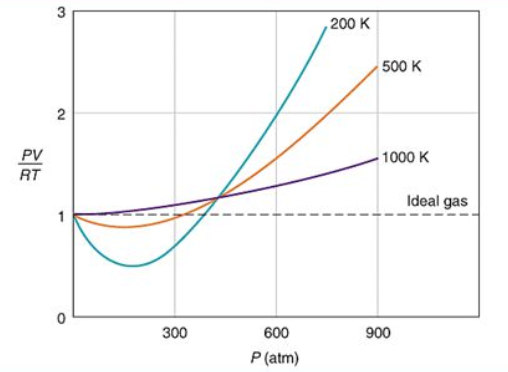
\includegraphics[scale=1.0]{FactorCompressT.png}
\end{center}
\end{exr}
\begin{exr}{Pressions parcials aire}
La composició percentual, en massa, de l'aire sec al nivell del mar és, aproximadament, \ch{N2}/\ch{O2}/\ch{Ar}=75.5/23.2/1.3. 
Quina és la pressió parcial de cada component quan la pressió total és 1.20 atm?.
\end{exr}
\lct{
En 100gr d'aire tindrem 75.5, 23.2 i 1.3 gr de \ch{N2}, \ch{O2} i \ch{Ar}, respectivament. Podem calcular la seva fracció molar calculant el número de mols de cadascun i dividint pel total. Després, només cal multiplicar per la pressió corresponent i sabrem la pressió parcial de cada component:

\[n_{\ch{N2}}=75.5 \cancel{g} \cdot \frac{1 mol}{28.02 \cancel{g}}=2.69 mol\]
\[n_{\ch{O2}}=23.2 \cancel{g} \cdot \frac{1 mol}{32.00 \cancel{g}}=0.725 mol\]
\[n_{\ch{Ar}}=1.3 \cancel{g} \cdot \frac{1 mol}{39.95 \cancel{g}}=0.033 mol\]

    \begin{tabular}{cccc}
      \hline
        & \ch{N2} & \ch{O2} & \ch{Ar} \\
      \hline
Fracció molar &	0.780 & 0.210 & 0.0096\\
Pressió parcial (nivell del mar)/atm & 0.780 & 0.210 & 0.0096\\
Pressió parcial ($P_T=1.20$atm))/atm & 0.936 & 0.252 & 0.012\\
      \hline
    \end{tabular}
}
 % Dalton
\begin{exr}
Una barreja de metà \ch{CH4} i d'acetilè \ch{C2H2} ocupava un cert volum a una pressió total de 63 mmHg. La mostra es va cremar a \ch{CO2} i \ch{H2O}. Se'n va recollir el \ch{CO2} en el mateix volum inicial i la mateixa temperatura inicial, i es va veure que la seva pressió era de 96 mmHg. Quina era la fracció de metà a la mescla de gasos inicials?
\end{exr}
\lct{
Definim $x$ com la fracció molar de metà (\ch{CH4}) i $y$ com la fracció molar d’acetilè (\ch{C2H2}):  
        \[
        x + y = 1
        \]
   
    Les reaccions de combustió són:
    
    \begin{align}
        \ch{CH4 + 2 O2 -> CO2 + 2 H2O}  & \quad \text{(1 mol de \ch{CH4} produeix 1 mol de \ch{CO2})} \\
        \ch{C2H2 + 5/2 O2 -> 2 CO2 + H2O}  & \quad \text{(1 mol de \ch{C2H2} produeix 2 mols de \ch{CO2})}
    \end{align}
    
    Si tenim un nombre total de mols $n$, llavors:
    
    \begin{itemize}
        \item Mols de metà: $xn$
        \item Mols d'acetilè: $yn$
    \end{itemize}
    
    Els mols de \ch{CO2} formats són:
    
    \[
    n_{\ch{CO2}} = xn + 2yn
    \]
     
    Com que el volum i la temperatura es mantenen constants, segons la llei dels gasos ideals la pressió és directament proporcional als mols:
      
    Així:
    
    \[
    P_{\ch{CO2}} = (xn + 2yn) \cdot \frac{P_{\text{total}}}{n}
    \]
    
    Substituint els valors donats:
    
    \[
    96 = (x + 2y) \cdot 63
    \]
    
   d'on
    
    \[
    x + 2y = \frac{32}{21}
    \]
    
   Ara ja podem resoldre el sistema:
    
    \begin{align}
        x + y &= 1 \\
        x + 2y &= \frac{32}{21}
    \end{align}
    
    i obtenim   
    \[
    x = 1 - \frac{11}{21} = \frac{10}{21}
    \]
    
    Per tant, la fracció de metà en la mescla inicial és:
    
    \[
    \frac{10}{21} \approx 0.476 \quad \text{o} \quad 47.6\%
    \]
}

\begin{exr}{Pressió parcial \ch{PCl5} en una mescla (adaptat de \cite{mahan_quimica_1997})}
    Una mostra de \ch{PCl5}, que pesa \SI{2.69}{\gram}, es va col·locar en un flascó d'\SI{1.00}{\litre} i es va evaporar completament a una temperatura de \SI{250}{\celsius}. La pressió observada a aquesta temperatura va ser \SI{1.00}{\atm}. Existeix la possibilitat que una part del \ch{PCl5} s'hagi dissociat d'acord amb l'equació:

\begin{reaction}
PCl5(g) -> PCl3(g) + Cl2(g)
\end{reaction}

Quines són les pressions parcials del \ch{PCl5}, \ch{PCl3} i \ch{Cl2} en aquestes condicions experimentals?
\end{exr}
\lct{
    La solució d'aquest problema implica diverses etapes. Per determinar si s'ha dissociat una part del \ch{PCl5}, calculem primerament la pressió que s'hauria observat si no s'hagués dissociat el \ch{PCl5}. Això es pot calcular a partir del nombre de mols de \ch{PCl5} utilitzats, juntament amb el volum i la temperatura del flascó. Com que el pes molecular del \ch{PCl5} és \SI{208}{\gram\per\mole}, el nombre de mols de \ch{PCl5} inicialment presents en el flascó és:

\[
n = \SI{2.69}{\gram}\cdot \frac{1\si{\mole}}{\SI{208}{\gram}} = 0.0129\si{\mole}.
\]

La pressió corresponent a aquest nombre de mols seria:

\[
P = \frac{nRT}{V} = \frac{(0.0129\si{\mole})(\SI{0.082}{\liter\atm\per\mole\per\kelvin})(\SI{523.15}{\kelvin})}{\SI{1.00}{\liter}} = \SI{0.553}{\atm}.
\]

Com que la pressió observada és superior a aquesta, s'ha de produir certa dissociació del \ch{PCl5}. Aplicant la llei de les pressions parcials, podem escriure:

\begin{equation}
P_{\ch{PCl5}} + P_{\ch{PCl3}} + P_{\ch{Cl2}} = P_t = \SI{1.00}{\atm}.
\label{eq:daltonpcl}
\end{equation}

Ara observem que:


Atès que es produeix un mol de \ch{PCl3} i un mol de \ch{Cl2} per cada mol de \ch{PCl5} dissociat,
\[
P_{\ch{Cl2}} = P_{\ch{PCl3}}, \quad P_{\ch{PCl5}} = \SI{0.553}{\atm} - P_{\ch{Cl2}}.
\]
i podem reescriure l'Equació \ref{eq:daltonpcl} com:

\[
\SI{0.553}{\atm} - P_{\ch{Cl2}} + P_{\ch{Cl2}} + P_{\ch{Cl2}} = \SI{1.00}{\atm}.
\]

Resolent, obtenim:

\[
P_{\ch{Cl2}} = \SI{0.447}{\atm},
\]

i

\[
P_{\ch{PCl3}} = \SI{0.447}{\atm}, \quad P_{\ch{PCl5}} = \SI{0.106}{\atm}.
\]
}

\begin{exr}
Perquè hi ha diferències entre els quocients de capacitat calorífica ($C_P/C_V$) de gasos monoatòmics respecte els diatòmics? (Adona't que si un gas monoatòmic ideal, pel fet d'estar només augmentant la seva energia cinètica translacional té una $C_V=\frac{3}{2}R$, es pot entendre que per a cada component (eix) necessita $\frac{1}{2}R$)
\end{exr}
\lct{
    Els quocients de la capacitat calorífica dels gasos diatòmics són molt menors que 1,67, i hem d'esbrinar la raó d'aquestes desviacions.

    Primerament, notem que $C_V$, la capacitat calorífica deguda al moviment de translació de les molècules, és igual a $\frac{3}{2}R$, i que hi ha tres components independents de velocitat associats amb el moviment de translació. Per tant, podem inferir que cadascun dels tres moviments de translació independents contribueix amb $\frac{1}{2}R$ a la capacitat calorífica molar. Sobre aquesta base, podríem esperar que, si algun altre tipus de moviment fos accessible a les molècules de gas, hi hauria més contribucions a la capacitat molar i aquestes entrarien en unitats de $\frac{1}{2}R$.
    
   A més de tenir els tres moviments de translació, una molècula diatòmica pot rotar al voltant del seu centre de massa segons dos modes mútuament perpendiculars i independents. Assignant $\frac{1}{2}R$ com la contribució de cadascun d'aquests moviments a la capacitat calorífica, tenim:
    
    \[
    C_V = \underbrace{\frac{3}{2}R}_{\text{traslació}} + \underbrace{\frac{1}{2}R + \frac{1}{2}R}_{\text{rotació}} = \frac{5}{2}R,
    \]
    
    \[
    C_P = C_V + R = \frac{7}{2}R,
    \]
    
    \[
    \frac{C_P}{C_V} = \frac{\frac{7}{2}R}{\frac{5}{2}R} = \frac{7}{5} = 1,40.
    \]
}

\begin{exr}
Qui es mou més ràpid, una molècula d'oxigen o una de nitrogen en dues mostres d'aquests gasos a la mateixa temperatura? Pots explicar perquè la pressió és independent de la natura de les molècules?
\end{exr}

\begin{exr}
Calcula la velocitat mitjana de les molècules d'hidrògen a 25\si\degreeCelsius.
\end{exr}
\begin{exr}
Considerant que no es comporta idealment, calcula la temperatura de \qty{10}{\mole} de monòxid de carboni (\ch{CO}) sotmesos a una pressió de \qty{5}{\kilo\pascal} en un volum de \qty{2}{\meter\tothe{3}}.
\end{exr}
\lct{
    L'equació de Van der Waals per gasos reals és:

    \[
    \left( P + \frac{n^2 a}{V^2} \right) (V - nb) = nRT
    \]
    
on $a$ i $b$ són constants que depenen de la naturalesa del gas. En el nostre cas:

\begin{itemize}
    \item Nombre de mols: \( n = 10 \) mol  
    \item Pressió: \( P = \qty{5}{\kilo\pascal} \cdot \frac{\qty{1}{\atm}}{\qty{101.325}{\kPa}} = \qty{0.0493}{\atm} \)  
    \item Volum: \( V = \qty{2}{\meter\tothe{3}} = \qty{2000}{\liter} \)  
    \item Constants de Van der Waals per \ch{CO}:
    \begin{itemize}
        \item \( a = \qty{1.4850}{\liter\squared\atm\per\mole\squared} \)
        \item \( b = \qty{0.03985}{\liter\per\mole} \)
    \end{itemize}
    \item Constant dels gasos: \( R = \qty{0.0821}{\liter\atm\per\mole\per\kelvin} \)
\end{itemize}

Calculem el terme de correcció de la pressió:

\[
    P + \frac{a n^2}{V^2} = 0.0493+\frac{(1.4850)(10)^2}{(2000)^2} = \qty{0.0493}{\atm}
\]


Calculem el volum corregit:

\[
V - nb = 2000 - (10 \times 0.03985) = 2000 - 0.3985 = \qty{1999.6}{\liter}
\]

Es pot veure com l'efecte de la no idealitat en aquest gas és molt reduït.  
Substituïm a l'equació:

\[
(0.0493)(1999.6) = (10)(0.0821)T
\]


\[
T = \frac{98.57}{0.821} = \qty{120}{\kelvin}
\]
}

\begin{exr}{Comportament no ideal d'un gas}
Perquè \ch{CO2} i \ch{O2} 
tenen una desviació negativa respecte al comportament del gas ideal a pressions i temperatures moderades, mentres que l'He i el 
\ch{H2} 
presenten una deviació positiva en les mateixes condicions?
\end{exr}
\lct{
    Els gasos \ch{CO2} i \ch{O2} presenten una desviació negativa respecte al comportament ideal perquè tenen interaccions intermoleculars atractives significatives. Aquestes forces atractives fan que, a pressions i temperatures moderades, les molècules s'acostin més del que prediu l'equació del gas ideal, reduint així el volum efectiu i fent que el factor de compressibilitat \( z = \frac{PV}{RT} \) sigui menor que 1.

D'altra banda, els gasos com l'heli (\ch{He}) i l'hidrogen (\ch{H2}) presenten una desviació positiva perquè tenen interaccions intermoleculars molt febles i, a mesura que augmenta la pressió, dominen els efectes de repulsió a causa del volum finit de les molècules. Això fa que el gas ocupi un volum lleugerament superior al que prediu el model ideal, fent que \( z > 1 \) en aquestes condicions.
}

%\begin{qst}
Fem una dissolució barrejant dos mols de metanol amb un mol d'etanol a una $T$ donada. Si la $P_v$ del metanol pur a aquesta $T$ és de 81 kPa, i la de l'etanol pur a la mateixa $T$ és de 45 kPa,
quina és la pressió de vapor de la barreja, assumint que és una dissolució ideal?
\end{qst}
\lct{
Hi ha 3 mols totals. Les fraccions molars són fàcilment calculables:
\[
x_{metanol}=2/3
\]
i 
\[
x_{etanol}=1/3
\]
Segons la llei de Raoult, la contribució a la pressió de vapor total de cada component ve donada pel producte de la seva fracció molar per la pressió de vapor de la substància pura:
\[
P_{metanol}=x_{metanol} \times P_{metanol}^0 = 2/3 \times 81 kPa = 54 kPa
\]
\[
P_{etanol}=x_{etanol} \times P_{etanol}^0 = 1/3 \times 45 kPa = 15 kPa
\]
Per tant, $P_{total}=P_{metanol}+P_{etanol}=54 kPa + 15 kPa = 69 kPa$
}
 % Raoult
%\begin{qst}
Perquè es generen bombolles de seguida que obrim una ampolla d'aigua amb gas?
\end{qst}
\lct{
Segons la llei de Henry, la concentració de gas en un líquid és proporcional a la pressió parcial externa d'aquest gas. Quan s'embotella  aigua carbonatada es fa a una pressió superior a 1 atm. Quan obrim l'ampolla, la pressió es redueix fins a 1 atm, i per tant el \ch{CO2} no és tan soluble i escapa de la dissolució formant bombolles.
} % Henry
%\begin{qst}
La constant de la llei de Henry de l'\ch{O2} en aigua a 25\si\degreeCelsius és 1.27·10$^{-3}$ M atm$^{-1}$, i la fracció molar de l'\ch{O2} en l'atmosfera és 0.21. Calcula la solubilitat de l'\ch{O2} en aigua a 25\si\degreeCelsius i a pressió atmosfèrica.
\end{qst}
\lct{
Segons la llei de Dalton, la pressió parcial d'un gas en una dissolució de gasos és proporcional a la seva fracció molar: $P_A=x_A P_t$. Per tant, $P_{\ch{O2}}=0.21 \times 1 atm=0.21 atm$. 

A partir de la llei de Henry, la concentració d'oxigen dissolt en les condicions donades és 
\[
[\ch{O2}]=k P_{\ch{O2}} = 1.27 \times 10^{-3}M atm^{-1} \cdot 0.21 atm=2.7 \cdot 10^{-4}M 
\]
}
 % Henry
%\begin{qst}{}
La $T$ de congelació del benzè pur és 5.40\si\degreeCelsius. 
Quan es dissol 1.15g de naftalè en 100 g de benzè, la dissolució resultant té un punt de congelació de 4.95\si\degreeCelsius.
Si la constant de descens molal del punt de congelació del benzè és 5.12\si\degreeCelsius, quin és el pes molecular del naftalè?
\end{qst}
\lct{
La molalitat de la dissolució és 
\[
m=\frac{\Delta T}{K_f} = \frac{5.40-4.95}{5.12}=0.088
\]
A partir de la quantitat de naftalè i la molalitat:
\[
\frac{\qty{1.15}{\gram}\,\text{ naft}}{ \qty{100}{\gram}\,\text{dissolv}} \cdot \frac{\qty{1000}{\gram}\,\text{dissolv}}{\qty{0.088}{\mole}\,\text{naft}} = \qty{130}{\gram\per\mole}
\]
}
 % solubilitat
%\begin{qst}
Calcular l'entalpia normal de formació de l'ió \ch{OH^-_{(aq)}} a partir de les següents calors de reacció:
\[
\begin{array}{cc}
\ch{1/2 O2_{(g)} + H2_{(g)} <-> H2O_{(l)}} & \Delta H^{\circ} = -285.9 kJ mol^{-1} \\
\ch{H2O_{(l)} <-> H^+_{(aq)} + OH^-_{(aq)}} & \Delta H^{\circ}=55.9 kJ mol^{-1}
\end{array}
\]
\end{qst}
\lct{
Només cal sumar les dues equacions per obtenir la reacció desitjada de formació dels dos ions, i sumem de la mateixa manera les calors de reacció:
\[
\begin{array}{cc}
\ch{1/2 O2_{(g)} + H2_{(g)} <-> H^+_{(aq)} + OH^-_{(aq)}} & \Delta H^{\circ} = -230.0 kJ mol^{-1} \\
\end{array}
\]
Com que la calor normal de formació de l'ió \ch{H+} és $\Delta H^{\circ}_f=0$, es dedueix que 
$\Delta H^{\circ}_f [\ch{OH^-_{(aq)}}= -230.0 kJ mol^{-1}$
} % entalpia de formació

\end{document}
